\section{Results}
\label{hptpcPaper:sec:Results}
Data and MC figures as a function of:
\begin{itemize}
    \item number of moderator blocks
    \begin{figure}[h]
        \centering
        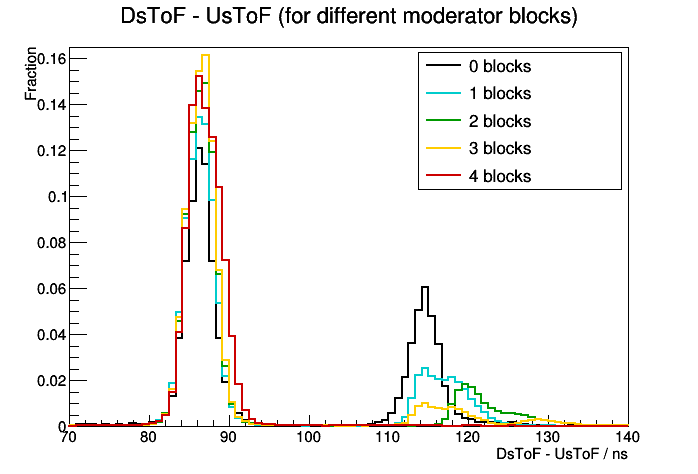
\includegraphics[width=0.7\linewidth]{files/Figures/AllInOne.png}
        \caption{Time of flight spectra for varying numbers of moderator blocks. For all configurations, the exposure has been normalised to one.}
        \label{fig:dtof_nmodblocks}
    \end{figure}
    \item Off axis angles
    \begin{figure}
        \centering
        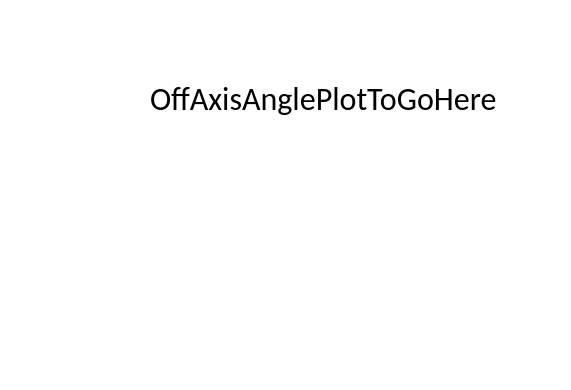
\includegraphics[width=0.7\linewidth]{files/Figures/OffAxisAngleDToFPlotToGoHere.png}
        \caption{Plot showing variation with respect to off axis angle of proton ratio, etc. in the DToF system}
        \label{fig:dtof_nmodblocks}
    \end{figure}
\end{itemize}
(Including absolute rates)

Exact UToF and DToF figures TBD